\chapter{Thiết kế}

\section{Mô hình thiết kế}
    Với mục tiêu đề tài giúp các quadcopter bay được ổn định đồng thời vẫn giữ được trạng thái bầy đàn nhóm đề xuất ra mô hình bay như sau:
    \begin{itemize}
    	\item Mô hình sẽ có ít nhất hai chiếc quadcopter có thể hoạt động độc lập ổn định. Như vậy cần có các cảm biến cần thiết để triển khai phương pháp điều khiển PID cho quadcopter. Ngoài ra còn cần mạch thu phát sóng Wifi và một vi xử lý phụ nhằm xử lý dữ liệu bay.
    	\item Trạm điêu khiển mặt đất chạy phần mềm để thiết lập thông số các quadcopter đồng thời hiển thị dữ liệu và điều khiển các quadcopter bay theo các chế độ mong muốn.
    	\item Mỗi chiếc quadcopter kết nối với trạm điều khiển đồng thời trao đổi dữ liệu cảm biến qua lại với nhau nhằm tính toán để giữ đội hình bầy đàn.
    \end{itemize}
    
    \begin{figure}[h!]
    	\begin{center}
    		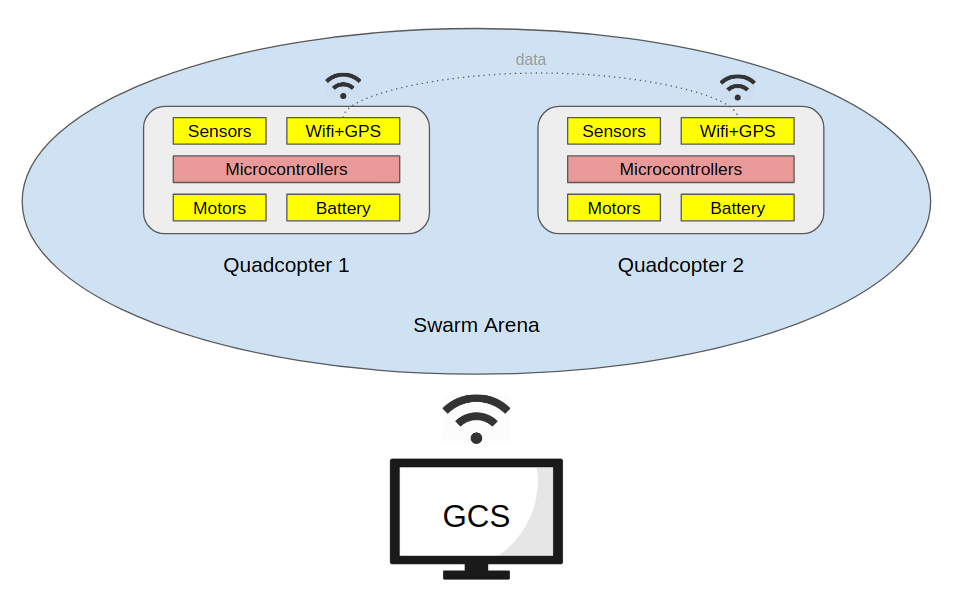
\includegraphics[scale=0.5]{images/design_model.png}
    		\caption{Mô hình thiết kế}
    	\end{center}
    \end{figure}
    
\section{Phần cứng} 
    \subsection{IMU - Đơn vị đo lường quán tính}
    \subsection{MCU - Vi điều khiển}
    \subsection{ESC - Bộ điều tốc}
    \subsection{ESP8266}
    \subsection{Ultrasonic Sensor - Cảm biến siêu âm}
   
   
    \section{Phần mềm}
            \subsection{S132 Softdevice}
        S132 Softdevice hiện thực các lớp trong mô hình BLE được viết cho chip nRF52832, hỗ trợ 4 vai trò trong giao thức BLE: Central, Peripheral, Broadcaster, Observer. Softdevice đã được build thành file nạp (.bin), người dùng nạp file vào và tương tác với lớp Softdevice này thông qua API được cung cấp. Nhóm sử dụng phiên bản Softdevice s132 v3.1.0\cite{softdevice}.
        \begin{figure}[h!]
        	\begin{center}
        		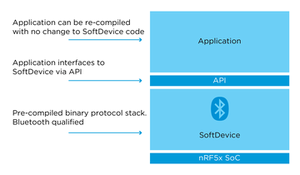
\includegraphics[scale=3.0]{images/SoC-Architecture_large.png}
        		\caption{Các lớp trong một chương trình}
        	\end{center}
        \end{figure}
        \subsection{nRFgo Studio}
        nRFgo Studio là chương trình dùng để nạp Softdevice cho các KIT phát triển, hỗ trợ nhiều chức năng liên quan đến Bluetooth, hiển thị trạng thái bộ nhớ hiện tại của chip,... 
        \subsection{Nordic Mesh SDK}
        Trong đề tài này, nhóm sử dụng nRF5 SDK for Mesh phiên bản v1.0.1 vì đây là phiên bản mới nhất vào thời điểm bắt đầu thực hiện luận văn. Ở thời điểm báo cáo luận văn thì Nordic đã cho ra mắt phiên bản v2.0.1 với một số thay đổi như: thêm chức năng provisioning thông qua GATT (PB-GATT), hỗ trợ chức năng Proxy cho các node và đặc biệt nhất: Mesh stack chính thức hoạt động ổn định. \\
        
        Ngoài ra còn có một số tính năng mà Nordic đang và sẽ cung cấp trong SDK này. Lưu ý: Một số tính năng chưa được hiện thực trong phiên bản SDK hiện tại.
            \begin{itemize}
                \item Device State Manager (DSM): DSM lưu trữ vào bộ nhớ flash những thông tin như Network key của mạng hiện tại, địa chỉ của các element,... Sau khi quá trình provisioning cho node mới hoàn tất, DSM sẽ lưu trữ thêm các thông tin của model, bao gồm địa chỉ và key để các model khác có thể giao tiếp với model này.
                \item Device Firmware Update (DFU): DFU giúp lập trình viên cập nhật firmware cho tất cả node trong mạng mà không cần tiếp xúc trực tiếp với từng node bằng cách áp dụng khả năng lan truyền của mesh.
                \item Hỗ trợ kết nối GATT/GAP, liên kết mạng mesh với các thiết bị như máy tính, điện thoại thông minh,...
                \item Serial, RTT: Cung cấp kênh giao tiếp giữa chip và máy tính, có thể truyền lệnh hay dữ liệu qua lại.
            \end{itemize}
            
        \subsection{Nordic SDK}
        SDK này cung cấp các API để người lập trình dễ dàng lập trình trên các dòng chip của Nordic, cụ thể là chip nRF52832 trong đề tài này. Tuy nhiên do phát triển không đồng thời với Mesh SDK nên khi sử dụng chung có thể gây ra xung đột, đặc biệt là các ứng dụng có dùng Softdevice vì đa phần các API của Nordic SDK không tương thích với Softdevice. Nhóm sử dụng Nordic nRF5 SDK v14.2.0\cite{nrf5sdk}.
    	\subsection{Thư viện giao tiếp module SIM}
    	Thư viện do nhóm tự phát triển và sử dụng trong một dự án trước đây, nhằm mục đích giao tiếp với module 3G SARA click. Thư viện có sẵn một số API cung cấp chức năng cơ bản như: khởi tạo, nghe gọi, xử lý tin nhắn, GPRS, HTTP request,... Trong đề tài này nhóm hiện thực thêm phần giao tiếp TCP để kết nối với cloud.
    	\subsection{ThingSpeak}
    	Nhóm sử dụng một cloud thông dụng dành cho các ứng dụng IoT giám sát đơn giản là ThingSpeak. Dữ liệu sau khi upload lên sẽ được hiển thị dạng biểu đồ và bất kỳ ai có liên kết đều có thể quan sát.
    	\subsection{Embedded Studio}
    	Chương trình hoàn toàn miễn phí, đóng vai trò IDE được Nordic khuyên dùng, các ví dụ được cung cấp trong các SDK đều được viết dưới dạng 1 project Segger Embedded Studio. Đặc biệt các project này đã cấu hình sẵn địa chỉ nạp để tránh đụng độ với Softdevice.
    
    
